% chapter5.tex
% Muon events, threshold analysis
Analysis of LED events can only be applied on the four extra top modules. To determine the stability of the total \mvs, aging of all modules are investigated. %In this chapter, the muon-events are selected and analysed. The efficiency change of each module are

\section{Analysis of Muon Events}


\begin{itemize}
  \item selection criteria,runs...
  \item Landau-spectrum, method detailed for M6..,   compare M8 with LED.
\end{itemize}

\subsection{Selection of muon-veto data}
All the data from Run70 (Aug 2010) to Run138 (Mar 2017) are investigated in the following analysis. First, data taken when the \mvs was not fully closed are cut. As described in \ref{sec:muon-setup}, two lasers measure the position of the upper part of muon-veto every 15 minutes. Time periods when the gap size deviates more than 5 cm from the closed configuration are cut, since \mvs is either fully closed or fully opened.
When \mvs is closed, most muons go through at least 2 modules. Therefore a coincidence in 2 distinct modules is required for selecting muon events.  An energy deposit with full informtaion in each module is required--i.e. both TDCs and ADCs have non-zero values.
It respectively reduces events caused by secondary particles or backgrounds since they mostly deposit less energy than muons.

\subsection{ }


\begin{figure}[ht]
  \centering
  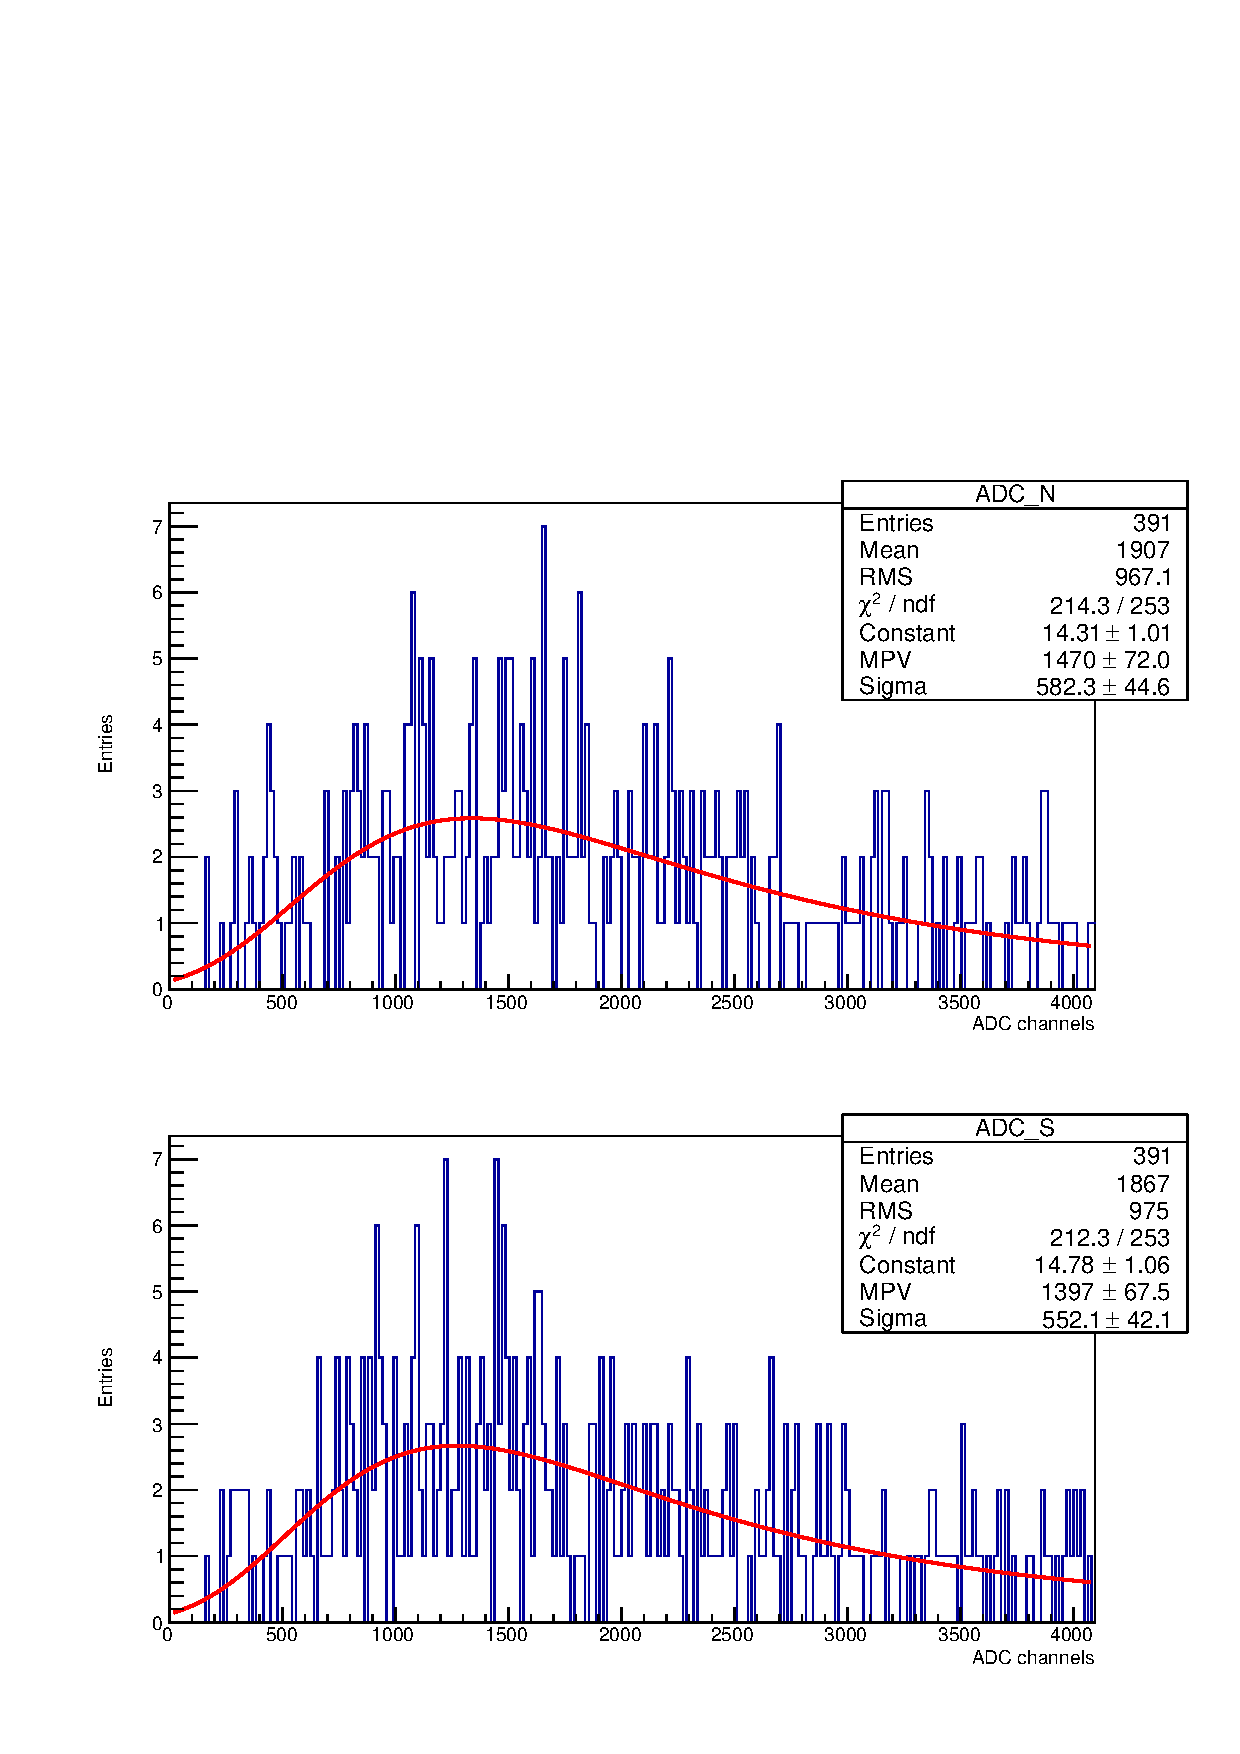
\includegraphics[width=0.7\textwidth{}]{./fig/LandauFitM6.pdf}
  \caption{Example of Landau spectrum in M6.}
  \label{fig:Landau_M6}
\end{figure}

\begin{figure}[ht]
  \centering
  \begin{subfigure}{0.5\linewidth}
    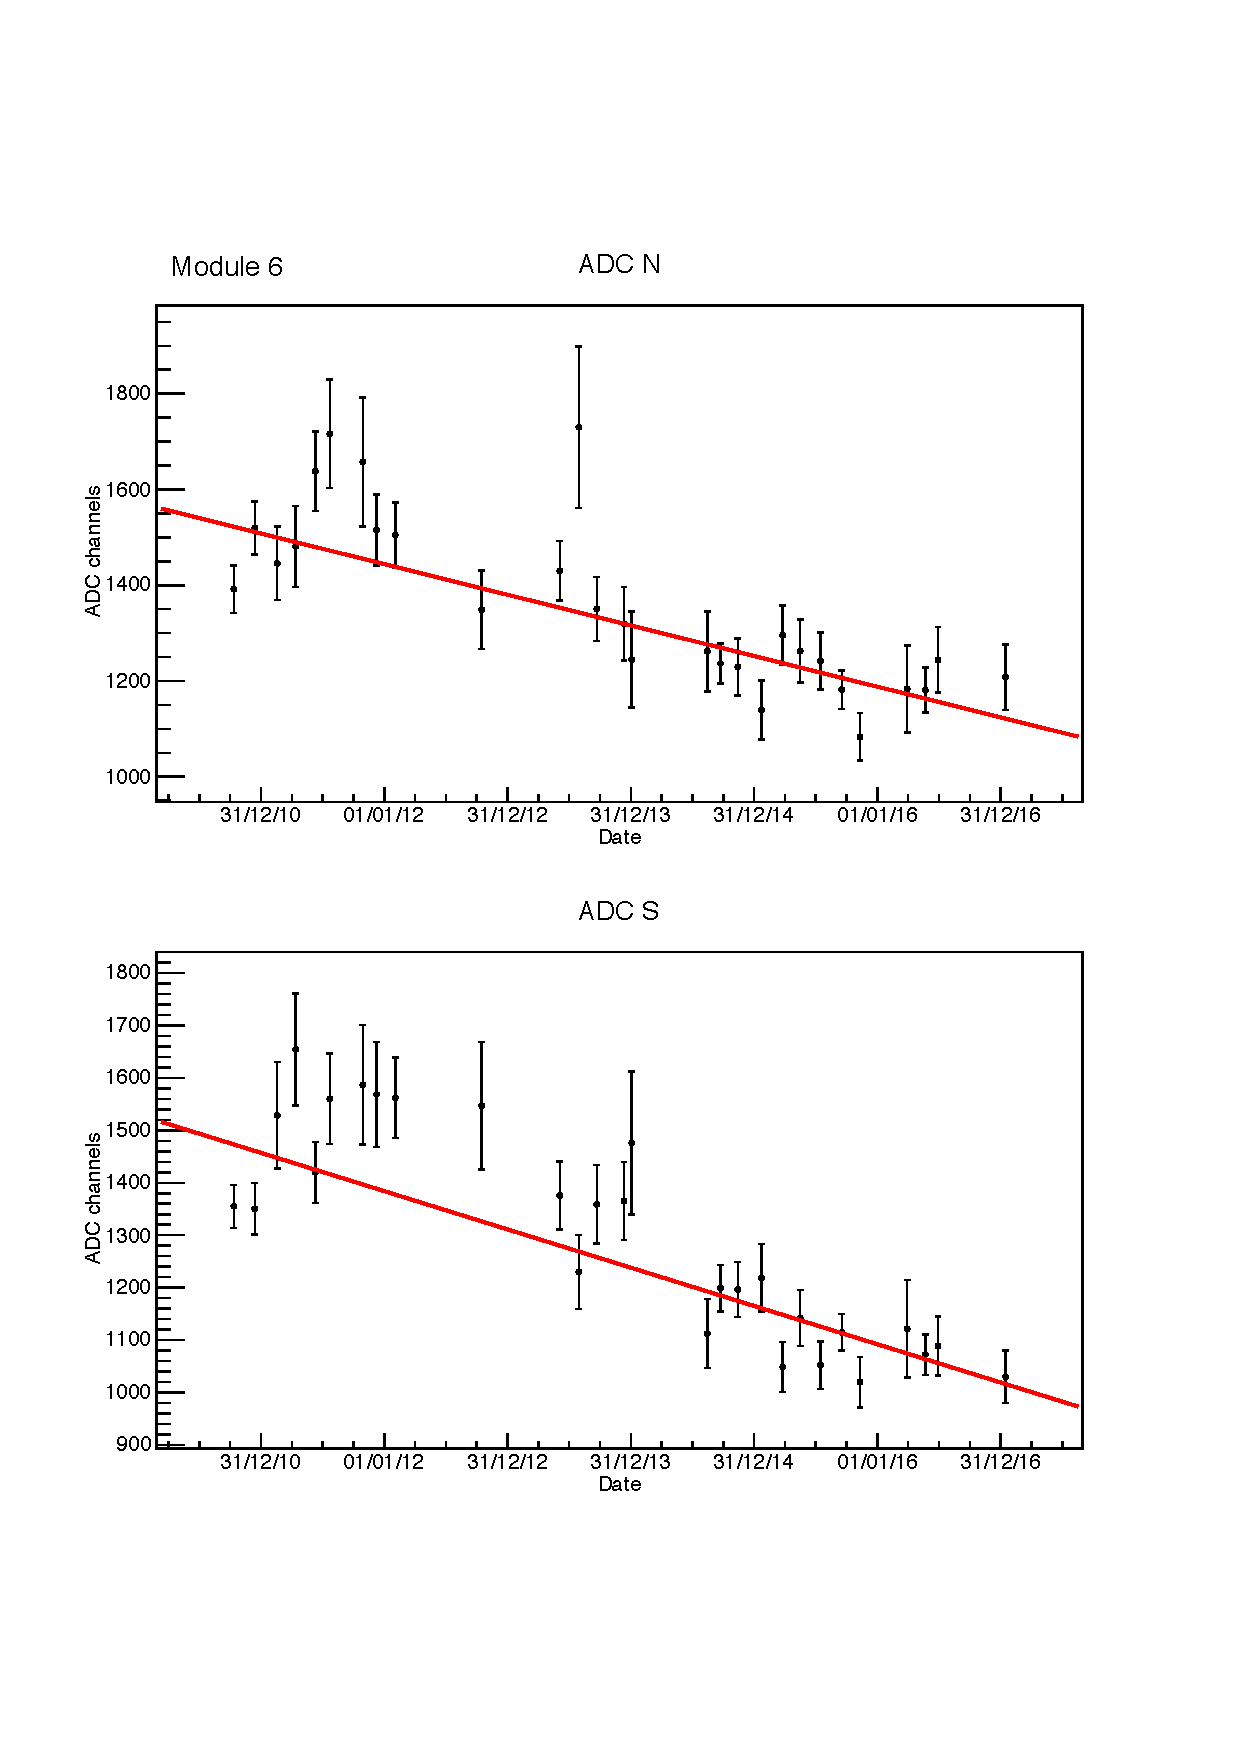
\includegraphics[width=\linewidth{}]{./fig/MPV_M6.pdf}
    \caption{}
    \label{fig:MPV_M6}
  \end{subfigure}
  \begin{subfigure}{0.5\linewidth}
    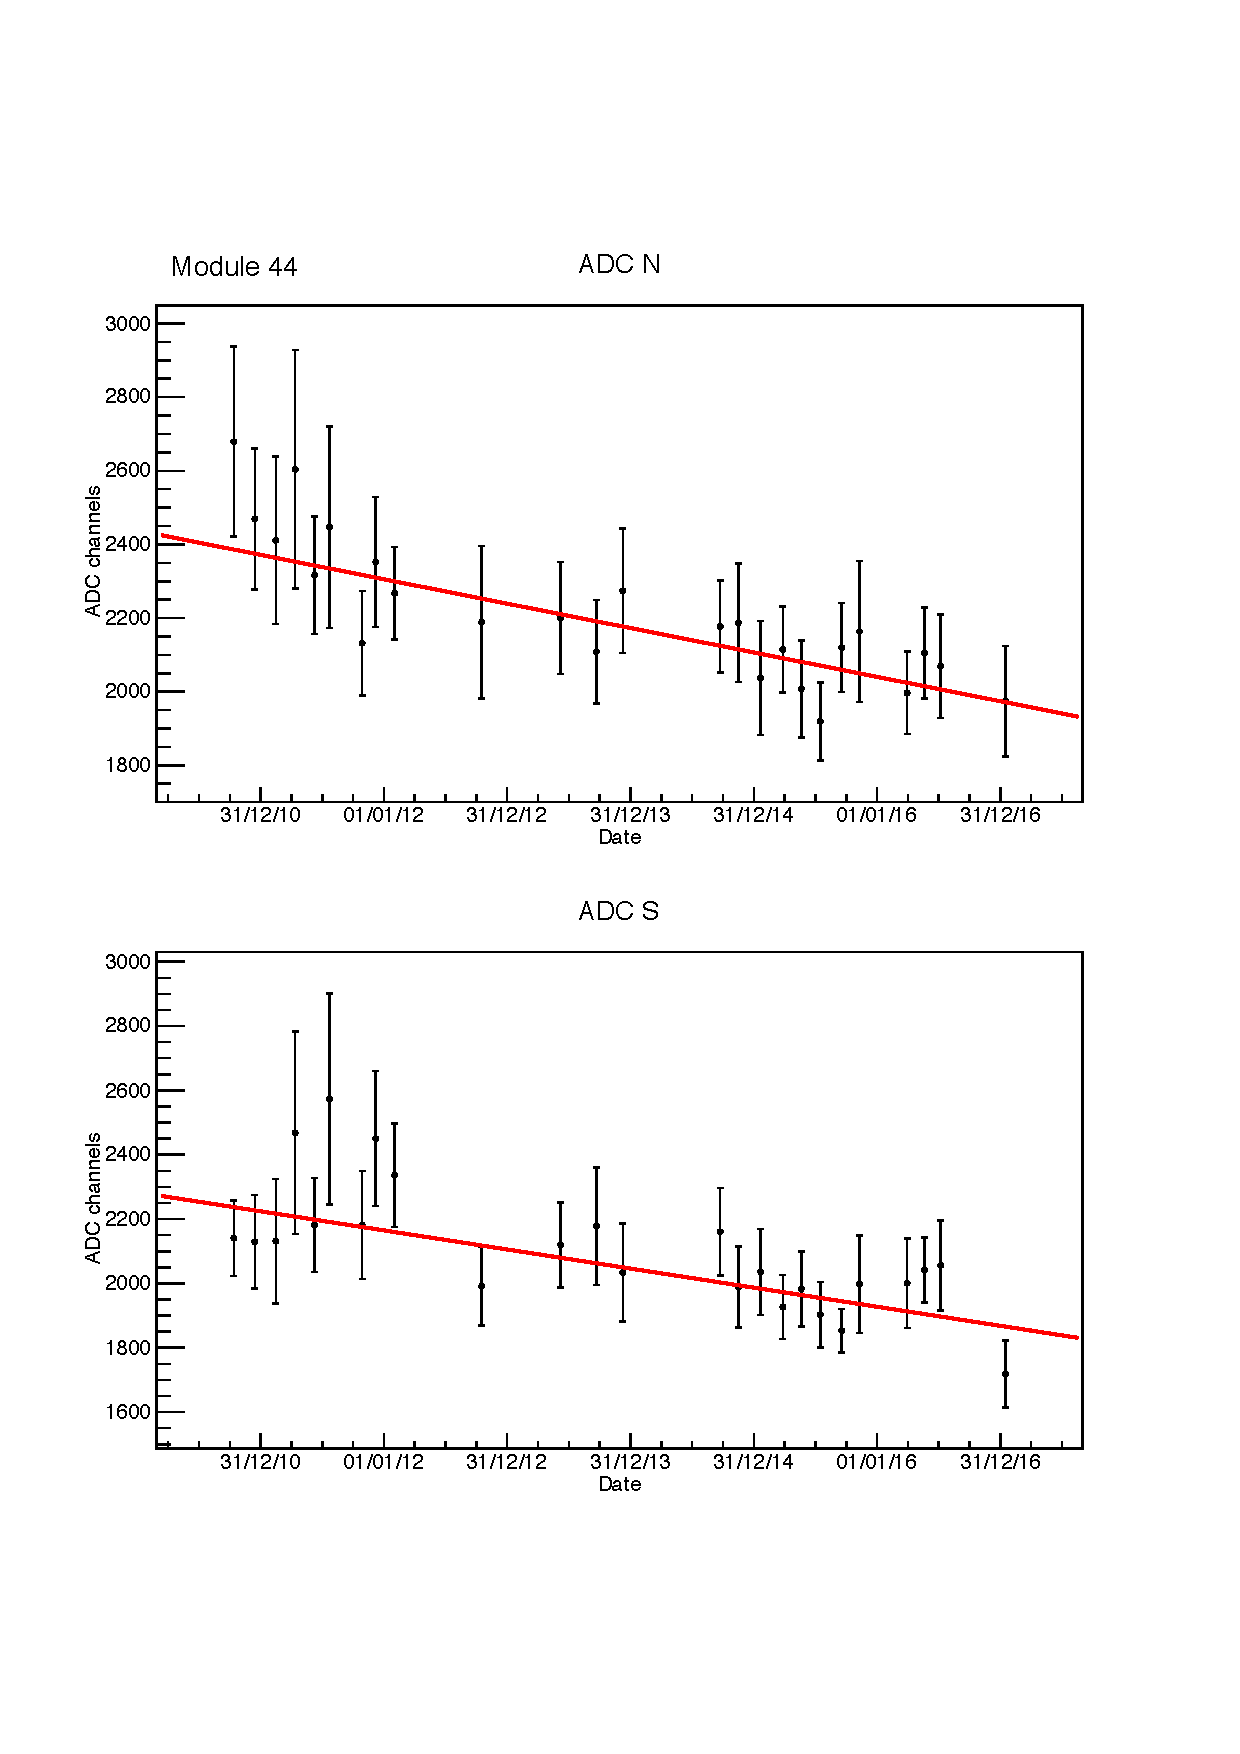
\includegraphics[width=\linewidth{}]{./fig/MPV_M44.pdf}
    \caption{}
    \label{fig:MPV_M44}
  \end{subfigure}
\end{figure}





\section{Determination of the detection efficiency}


\begin{itemize}
  \item conversion threshold,effective threshold
  \item method to determine threshold
  \item result, change of efficiency
\end{itemize}

\begin{figure}[ht]
  \centering
  \begin{subfigure}{0.7\linewidth}
    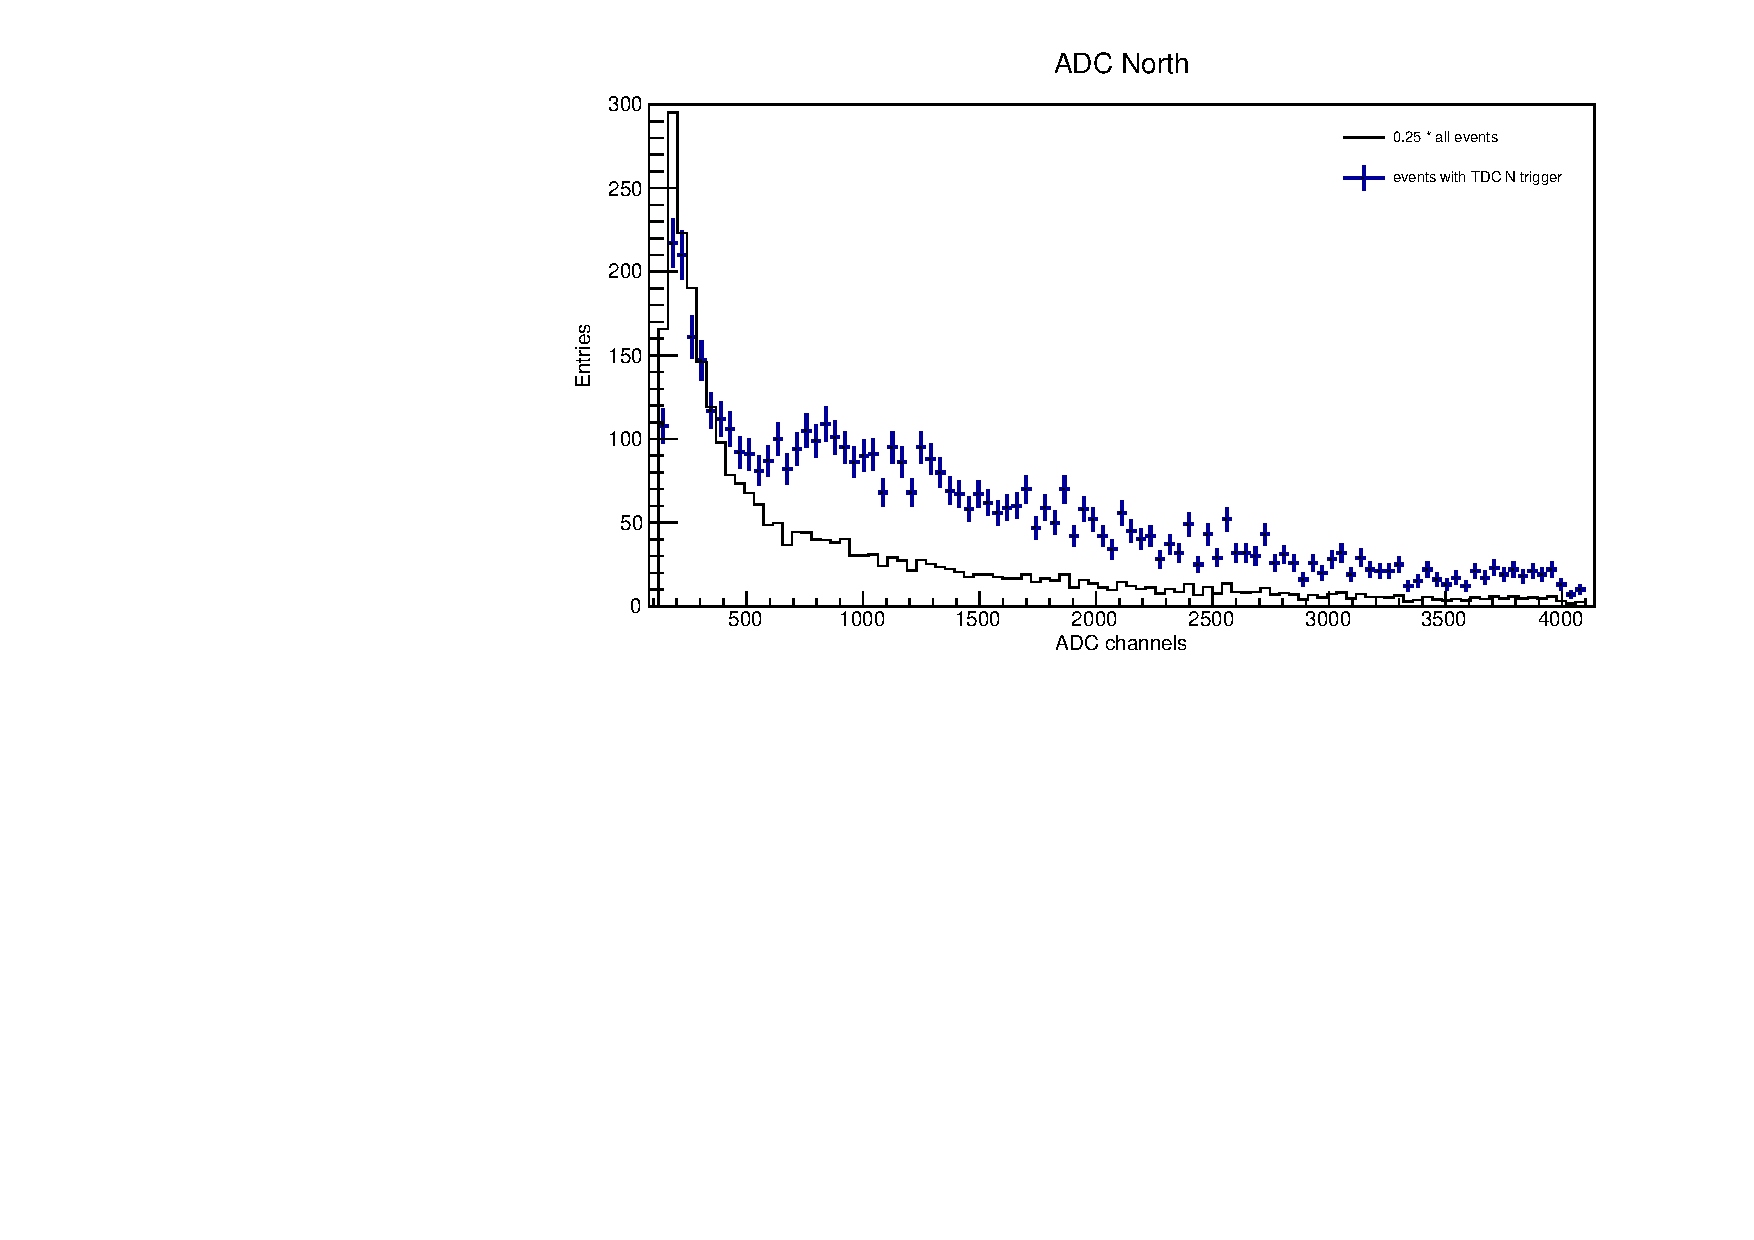
\includegraphics[width=\linewidth{}]{./fig/M6AdcNorth2Histo.pdf}
    \caption{}
    \label{fig:2HistoM6}
  \end{subfigure}
  \begin{subfigure}{0.7\linewidth}
    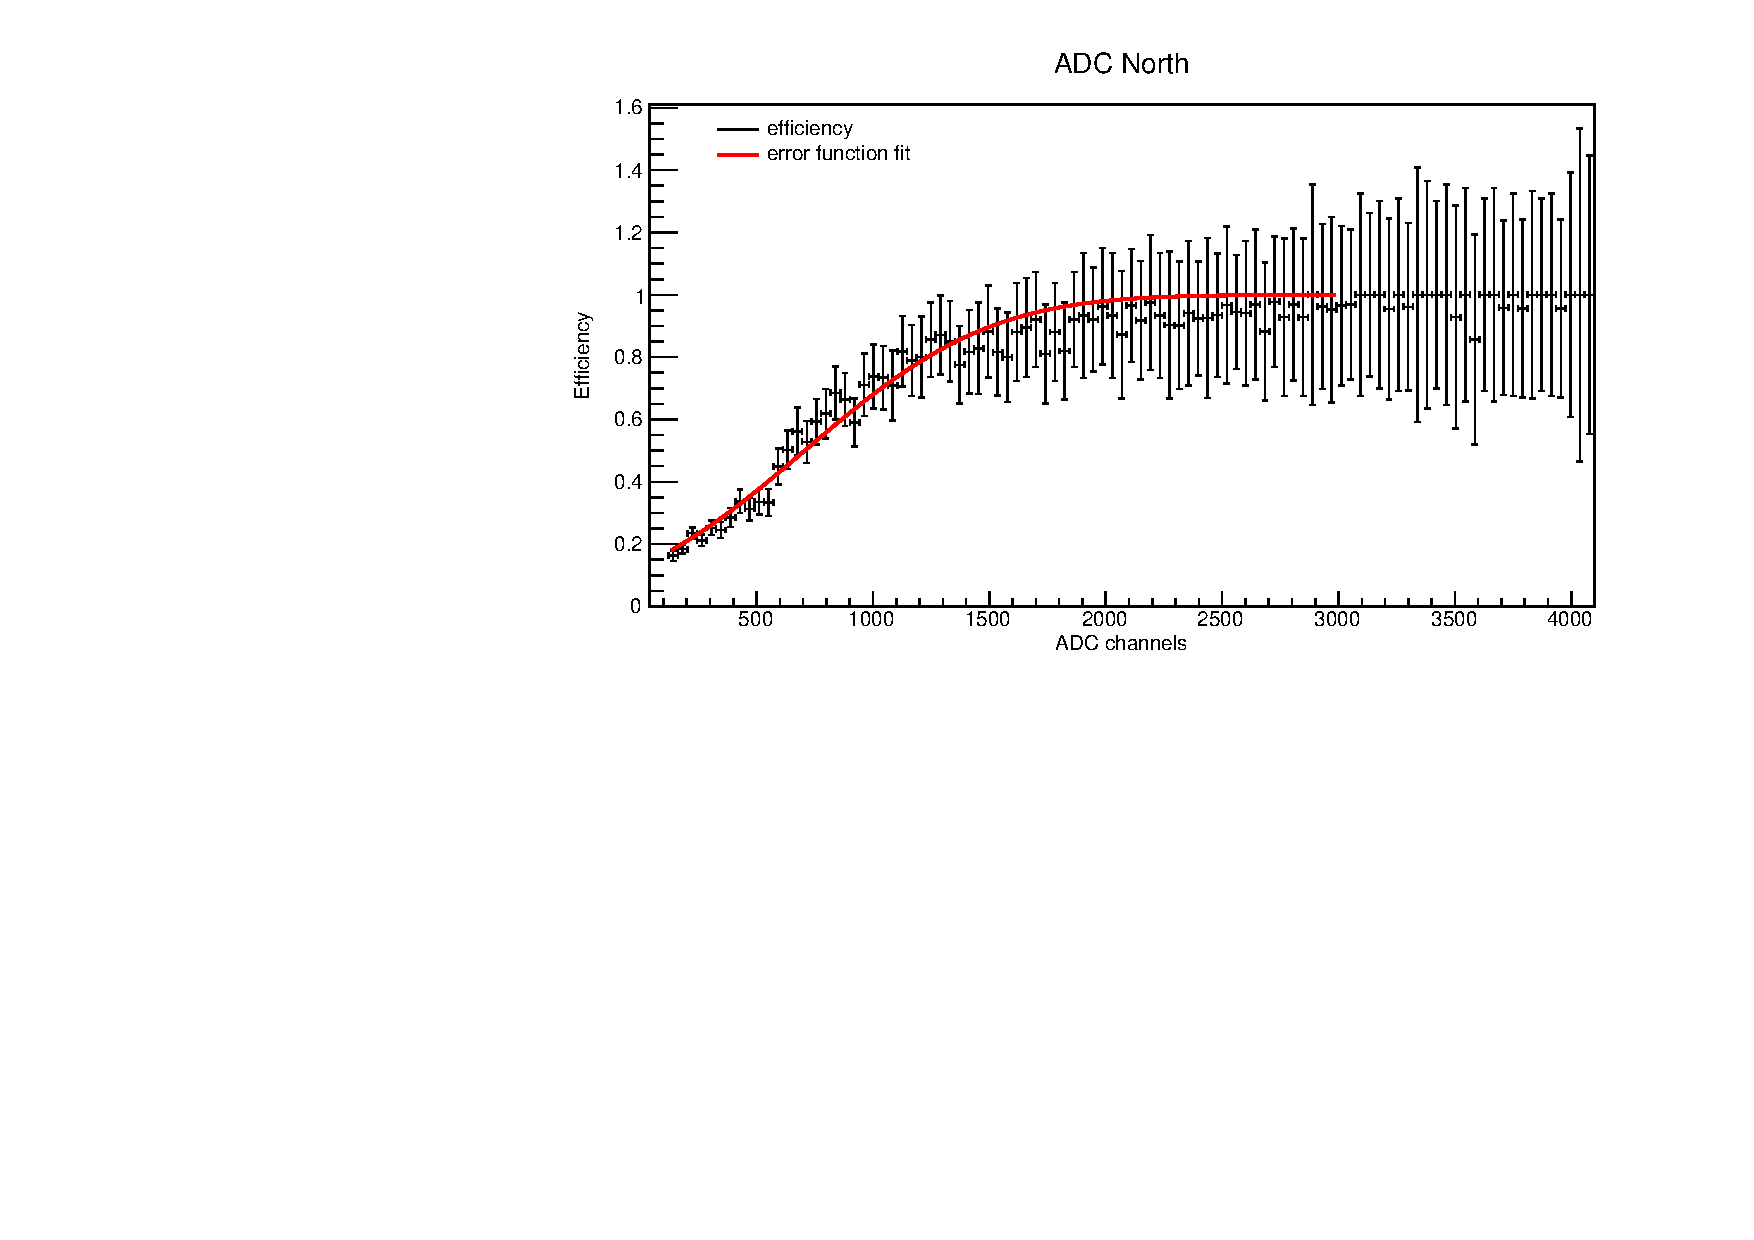
\includegraphics[width=\linewidth{}]{./fig/M6AdcNortheff_late.pdf}
    \caption{}
    \label{fig:eff_lateM6}
  \end{subfigure}
\end{figure}
